%%%%%%%%%%%%%%%%%%%%%%%%%%%
% 論文風格
%%%%%%%%%%%%%%%%%%%%%%%%%%%
\documentclass[hyperref,UTF8,12pt,a4paper]{ncku-style/ncku_class}
\usepackage{ncku-style/style}

%%%%%%%%%%%%%%%%%%%%%%%%%%%
% 論文參數
%%%%%%%%%%%%%%%%%%%%%%%%%%%
\usepackage{thesis-param/Date}
\usepackage{thesis-param/DepartmentInfomation}
\usepackage{thesis-param/TableOfContent}
\usepackage{thesis-param/Title}
\usepackage{thesis-param/Writer}

%%%%%%%%%%%%%%%%%%%%%%%%%%%
% 套件引用
%%%%%%%%%%%%%%%%%%%%%%%%%%%
\usepackage{fancyhdr}  % 借用此套件來擺放浮水印,產生 header, footer
\pagestyle{fancy} % 啟動 fancy header/footer 套件
\fancyhead{}  % reset left, central, right header to empty
\fancyfoot[C]{\thepage} % 中間 footer 擺放頁碼
\renewcommand{\headrulewidth}{0pt} % header 的直線; 0pt 則無線
\usepackage{CJKutf8}  % macro for Chinese/Japanese/Korean processing
\usepackage{CJKnumb}  % for Chinese numbering capability
\usepackage{type1cm}
\usepackage{indentfirst}
\usepackage[pdftex]{graphicx}
\newcommand\myworkflow{pdftex}  % set the flag
\usepackage{hyperref}
\hypersetup{unicode,colorlinks,
    citecolor=black,
    filecolor=black,
    linkcolor=black,
    urlcolor=black}
\usepackage{graphicx} \graphicspath{{images/}}
\usepackage{psfrag} % text replacement in figure
\usepackage{bm}
\usepackage{mathtools}
\usepackage{float}
\floatstyle{plaintop}
\restylefloat{table}
\usepackage[T1]{fontenc} 
\usepackage{newtxmath,newtxtext}
\usepackage{titletoc} % handling toc/lof/lot entries
\usepackage[]{titlesec} % 分段命令提供自定義選項(將chapter1修改爲第1章)
\usepackage[usenames,dvipsnames,table]{xcolor}
\usepackage{url} % 引用網址 \url{http://www.yzu.edu.tw}
\usepackage{ragged2e} % 增強版文本對齊選項
\usepackage{caption} % 自定義圖形和表格標題
\captionsetup[figure]{labelsep=space, justification=centering, singlelinecheck=false}
\captionsetup[table]{labelsep=space, justification=centering, singlelinecheck=false}
\usepackage{subcaption} % 自定義圖形和表格子標題

%%%%%%%%%%%%%%%%%%%%%%%%%%%
% 文件設定
%%%%%%%%%%%%%%%%%%%%%%%%%%%
\begin{document}
\begin{CJK}{UTF8}{bkai} % 預設中文字型、編碼、標楷體
\CJKindent  % (global CJK setting)段首內縮兩格
% 針對 latex + dvipdfmx 工作流程在 hyperref 套件的影響下,圖檔的辨識力退化
% 所作的權宜措施。可能是因為 TeXLive2007 hyperref 裏的
% 客製 graphicx / dvipdfmx 的設定檔不夠新
\ifx\myworkflow\mydvipdfmxflow
	\DeclareGraphicsExtensions{.pdf,.png,.jpg,.eps}
	\DeclareGraphicsRule{.pdf}{eps}{.bb}{}
	\DeclareGraphicsRule{.png}{eps}{.bb}{}
	\DeclareGraphicsRule{.jpg}{eps}{.bb}{}
\fi
\renewcommand\prechaptername{第} % 出現在每一章的開頭的「第 x 章」
\renewcommand\postchaptername{章}
\newcommand{\tablename}{表} % 在文章中 table 會以「表 x」表示
\newcommand{\figurename}{圖} % 在文章中 figure 會以「圖 x」表示
\newcommand{\boldtext}{\fontseries{bx}\selectfont}
\newcommand{\Ssd}[1]{(#1)\hspace{0.8em}}
\renewcommand{\thesection}{\arabic{chapter}.\arabic{section}}
\renewcommand{\thesubsection}{\arabic{chapter}.\arabic{section}.\arabic{subsection}}
\titleformat{\chapter}{\centering\Large\bfseries\boldtext}{第\,\CJKnumber{\thechapter}\,章}{1em}{}
\titlespacing{\chapter}{0pt}{-20pt}{10pt}
\titleformat{\section}{\RaggedRight\large\bfseries\boldtext}{\,\thesection\,}{1em}{}
\titleformat{\subsection}{\RaggedRight\large\bfseries\boldtext}{\,\thesubsection\,}{1em}{}
\titleformat{\subsubsection}{\RaggedRight\bfseries\boldtext}{}{1em}{}

%%%%%%%%%%%%%%%%%%%%%%%%%%%
% 論文內容 
%%%%%%%%%%%%%%%%%%%%%%%%%%%
% 1. 封面頁
\NckuCoverPage

% 2. 口委中英文簽名單
% 手動利用 ilovepdf 網站合併至 PDF

% Roman 頁碼起始
\newpage
\setcounter{page}{1}
\pagenumbering{Roman}

% 3. 中英文摘要
\NckuZhAbstractPage
\NckuEnAbstractPage

% 4. 誌謝
\NckuAcknPage

% 5. 目錄
\NckuTOC

% 6. 表目錄
\NckuLOT

% 7. 圖目錄
\NckuLOF

% arabic 頁碼起始
\newpage
\setcounter{page}{1}
\pagenumbering{arabic}

% 8. Contents
% Function:
% (中文粗體) \highlight{}
\newcommand{\highlight}{\fontseries{bx}\selectfont\noindent}
% \newcommand{\redtext}[1]{\textcolor{red}{#1}}

\chapter{\chOneTitle}\section{研究動機}
隨著時間的推移,保持健康且高效的勞動力變得愈加困難,導致該行業面臨日益嚴重的缺工問題(圖\ref{fig:example_tag})。

\begin{figure}[H]
    \centering
    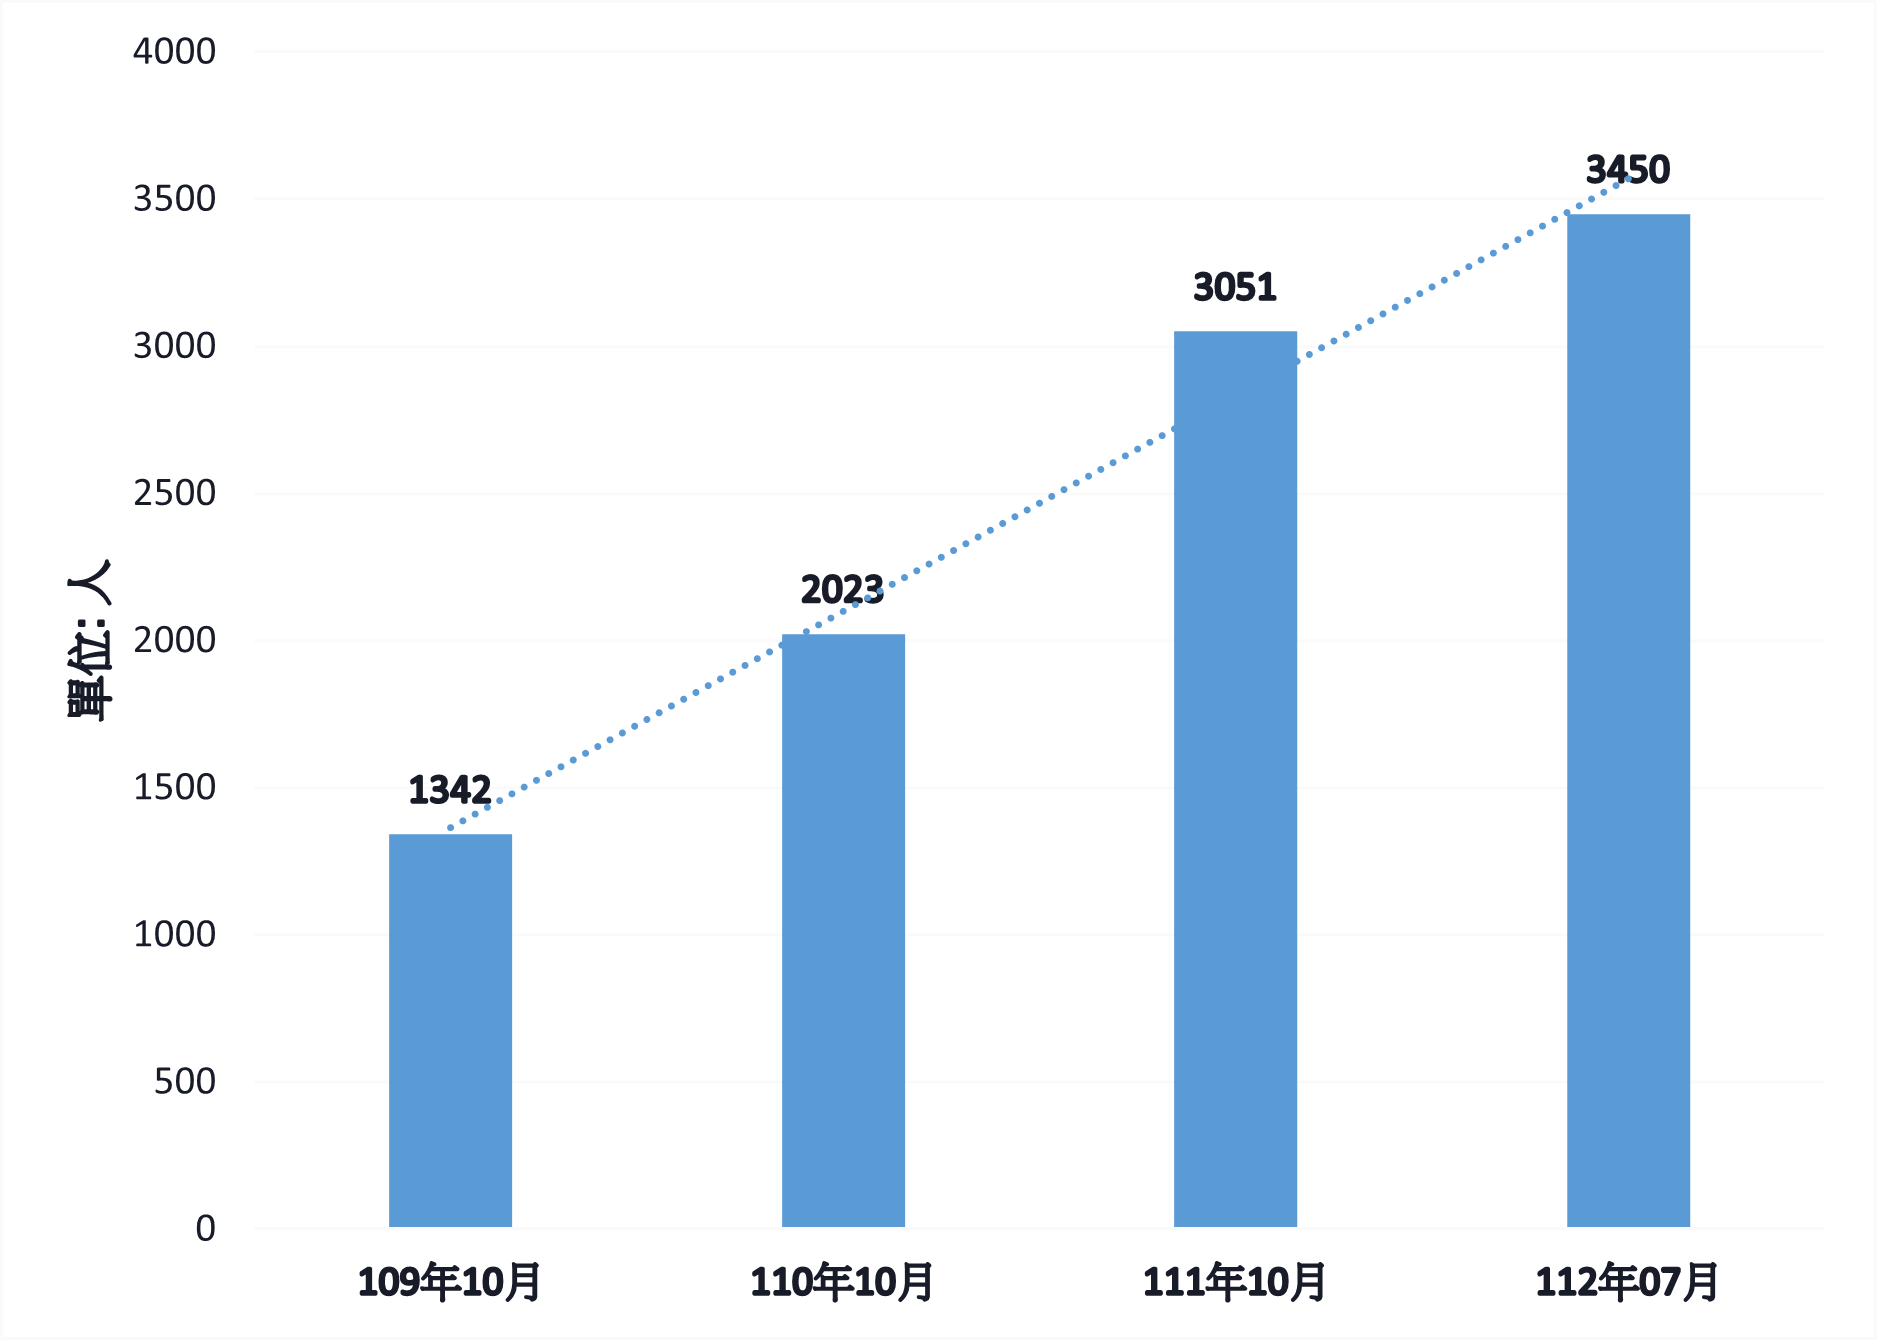
\includegraphics[width=10cm]{images/example.png}
    \caption{近四年營建工程業人力需求淨增減人數}
    \label{fig:example_tag}
\end{figure}

\section{研究目的}
解釋引入人機協作流程及數位雙生平台在建築營造行業中發展全自動化機器人的重要性,接著闡述研究目的和研究問題,並概述後續章節的內容。

\subsection{機器人於工地全自動化施作瓶頸}
解釋引入人機協作流程及數位雙生平台在建築營造行業中發展全自動化機器人的重要性,接著闡述研究目的和研究問題,並概述後續章節的內容。

\subsubsection{\Ssd{1}解析協作機器人位移規劃之資訊與操控需求} % ssd = subsubsection decoration
解釋引入人機協作流程及數位雙生平台在建築營造行業中發展全自動化機器人的重要性,接著闡述研究目的和研究問題,並概述後續章節的內容。

\subsubsection{第一章:緒論}
解釋引入人機協作流程及數位雙生平台在建築營造行業中發展全自動化機器人的重要性,接著闡述研究目的和研究問題,並概述後續章節的內容。

{\highlight 第一章:緒論}\\ % no indent and small padding in y direction
解釋引入人機協作流程及數位雙生平台在建築營造行業中發展全自動化機器人的重要性,接著闡述研究目的和研究問題,並概述後續章節的內容。

{\highlight 第一章:緒論} % have indent and small padding in y direction

解釋引入人機協作流程及數位雙生平台在建築營造行業中發展全自動化機器人的重要性,接著闡述研究目的和研究問題,並概述後續章節的內容。

\section{研究目的}

\subsubsection{\Ssd{1}解析協作機器人位移規劃之資訊與操控需求}

\subsubsection{\Ssd{2}改善建築資訊模型應用方法}

\subsubsection{\Ssd{3}建構數位雙生的人機協作平台}

\subsubsection{\Ssd{4}蒐集用於人工智慧訓練的虛實整合資料}
\chapter{\chTwoTitle}\allowdisplaybreaks[4]

第二章內容
\chapter{\chThreeTitle}\allowdisplaybreaks[4]

第三章內容	
\chapter{\chFourTitle}\allowdisplaybreaks[4]

第四章內容

\section{研究架構}

傳統自動導引車和自主移動機器人之間的差異如表 \ref{tab:compare-agv-amr} 所示,自動導引車不適用於工程現地主要原因為營建工程缺乏固定的生產線結構,機器人必須具有自由移動和具自適應性的能力。table 可以使用 latex table generator 產生,不必自己打!可參考這個 https://www.tablesgenerator.com/

\begin{table}[H]
    \centering
    \caption{AGV 和 AMR 間的差異比較}
    \label{tab:compare-agv-amr}
    \begin{tabular}{lll}
    \hline
    \rowcolor[HTML]{C0C0C0} 
    項目\hspace{1.5cm} & Automated Guided Vehicle & Autonomous Mobile Robot \\ \hline
    導航方式 & 固定路線 & 自主導航 \\
    預置設施 & 需要安裝 & 無需安裝 \\
    適用場景 & 固定環境 & 動態環境 \\ \hline
    任務性質 & 專注單一 & 多樣靈活 \\
    任務適應性 & 缺乏調整彈性 & 具可擴展性 \\
    導入速度 & 較長佈署時間 & 快速導入 \\ \hline
    \end{tabular}
\end{table}

URDF 文件以 XML 格式編寫,提供一種結構化的方式來定義機器人的各種組件。以下是本研究在創建自主移動平台的虛擬分身使用的重點 XML 標記及其用途:

\begin{itemize}
    \item <robot> 標籤:所有機器人組件必須在標籤內定義。
    \item <link> 標籤:每個標籤定義特定鏈接的視覺表示、碰撞屬性和慣性屬性。
    \item <joint> 標籤:原點(位置和方向)以及旋轉或平移軸,詳細類型見表 \ref{tab:urdf}。
    \item <collision> 標籤:在標籤內可以定義碰撞幾何並指定原點和摩擦係數等屬性。
    \item <inertial> 標籤:該標籤允許指定鏈接的質量、慣性矩和質心偏移。
    \item <visual> 標籤:材料(顏色和紋理)和原點(位置和方向)等屬性。
    \item <limit> 標籤:透過標籤規定關節運動的限制,可以定義限制屬性。
\end{itemize}

\begin{table}[H]
    \centering
    \caption{URDF 模型中的 joint 類型}
    \label{tab:urdf}
    \begin{tabular}{ll}
    \hline
    \rowcolor[HTML]{C0C0C0} 
    關節類型    & 描述                                          \\ \hline
    Continuous & 旋轉關節,繞軸承旋轉沒有旋轉上下限限制。            \\
    Revolute   & 旋轉關節,與 Continuous 相似,但有旋轉之限制範圍   \\
    Prismatic  & 滑動關節,沿軸向滑動,具有指定的限定範圍。          \\ \hline
    Planar     & 平移關節,允許在垂直於軸向的平面內進行移動。         \\
    Floating   & 自由關節,允許所有軸向上的運動(6個自由度)。        \\
    Fixed      & 固定關節,不能移動,所有自由度都被鎖定。            \\ \hline
    \end{tabular}
\end{table}

\section{人工智慧訓練資料蒐集流程}

資料是人工智慧模型的基礎,而高品質和多樣性的資料是訓練出準確、可靠模型的關鍵。然而在營建產業相關的數據資料集相當稀缺,主要受到數據保密性、資料碎片化、數據收集成本等因素,詳見表 \ref{tab:datamissing}。

\begin{table}[H]
    \centering
    \caption{營建產業資料集稀缺因素}
    \label{tab:datamissing}
    \begin{tabular}{ll}
    \hline
    \rowcolor[HTML]{C0C0C0} 
    因素     & 描述       \\ \hline
    數據保密性  & \begin{tabular}[c]{@{}l@{}}在建築營造領域,一些數據可能受到法律或商業機密的保護,\\ 例如高科技廠房,限制了數據的公開和分享,導致部分重要數\\ 據無法公開使用及獲取。\end{tabular} \\ \hline
    資料碎片化 & \begin{tabular}[c]{@{}l@{}}建築營建領域涉及多個相關腳色,包括業主、建築師、工程師\\ 、承包商、供應商等。相關方之間的數據通常以不同的格式和\\ 結構保存,並存儲在不同的系統和文件中。這導致數據碎片化\\ 使得整合和標準化變得困難。\end{tabular} \\ \hline
    數據收集成本 & \begin{tabular}[c]{@{}l@{}}在建築營建領域數據的收集需要耗費大量的時間、資源和成本\\ 。例如進行現場測量、監測和數據記錄需要人力和設備投入\\ ,限制了數據蒐集的規模和可用性。\end{tabular} \\ \hline
    \end{tabular}
\end{table}	
\chapter{\chFiveTitle}\allowdisplaybreaks[4]

第五章內容

第一種方式是使用系統分配的序列埠名稱。當傳感器連接到 USB 接口,系統會自動分配一個名稱,例如 $/dev/ttyUSB0$、$/dev/ttyUSB1$、$/dev/ttyUSB2$ 等,以區分不同的串行設備。該方式簡單直觀,通過查看 $/dev$ 目錄下的檔案,即可確定硬體連接之序列埠名稱,然而當系統中存在多個串行設備時,需要進行名稱映射或手動配置,例如傳感器的連接順序發生變化或重新插拔,名稱可能發生變更,導致需要重新為設備手動調整配置。

第二種方式是使用 $/dev/serial/by-id$ 目錄下的序列埠名稱。每個串接設備都有一個獨特的唯一識別符號,系統根據此識別符號在 $/dev/serial/by-id$ 建立對應的連接埠名稱,確保了名稱的唯一性。這種方式不受設備連接順序的影響,即使重新插拔設備,名稱也不會改變。因此,本研究選擇使用基於唯一識別符號的方式來指定設備的序列埠,以維持系統的穩定性。 

\section{實驗場域}

為了驗證混合實境之人機協作資料蒐集流程的可行性,本研究利用成功大學某教學大樓之室內空間做為案例驗證場域,建築相關資訊如下:

\begin{itemize}
  \item 建物名稱:成功大學某教學大樓
  \item 建物規模:鋼筋混凝土建築結構,地下兩層、地上七層
  \item 案例驗證空間:2F 指定區域
\end{itemize}

\chapter{\chSixTitle}\allowdisplaybreaks[4]

第六章內容
\chapter{\chSevenTitle}參考文獻使用 Microsoft Word 搭配 ASCE (老師偏好的引用格式) citation generator 撰寫,接著透過 ilovepdf 網站合併 PDF (https://www.ilovepdf.com/zh-tw/organize-pdf)

% 9. 參考文獻
% 手動利用 ilovepdf 網站合併至 PDF (注意頁碼)

\clearpage % to make sure all CJK characters are processed
\end{CJK}
\end{document}